\documentclass[]{article}
\usepackage{lmodern}
\usepackage{amssymb,amsmath}
\usepackage{ifxetex,ifluatex}
\usepackage{fixltx2e} % provides \textsubscript
\ifnum 0\ifxetex 1\fi\ifluatex 1\fi=0 % if pdftex
  \usepackage[T1]{fontenc}
  \usepackage[utf8]{inputenc}
\else % if luatex or xelatex
  \ifxetex
    \usepackage{mathspec}
  \else
    \usepackage{fontspec}
  \fi
  \defaultfontfeatures{Ligatures=TeX,Scale=MatchLowercase}
\fi
% use upquote if available, for straight quotes in verbatim environments
\IfFileExists{upquote.sty}{\usepackage{upquote}}{}
% use microtype if available
\IfFileExists{microtype.sty}{%
\usepackage{microtype}
\UseMicrotypeSet[protrusion]{basicmath} % disable protrusion for tt fonts
}{}
\usepackage[margin=1in]{geometry}
\usepackage{hyperref}
\hypersetup{unicode=true,
            pdftitle={homework2},
            pdfauthor={Laha Ale},
            pdfborder={0 0 0},
            breaklinks=true}
\urlstyle{same}  % don't use monospace font for urls
\usepackage{color}
\usepackage{fancyvrb}
\newcommand{\VerbBar}{|}
\newcommand{\VERB}{\Verb[commandchars=\\\{\}]}
\DefineVerbatimEnvironment{Highlighting}{Verbatim}{commandchars=\\\{\}}
% Add ',fontsize=\small' for more characters per line
\usepackage{framed}
\definecolor{shadecolor}{RGB}{248,248,248}
\newenvironment{Shaded}{\begin{snugshade}}{\end{snugshade}}
\newcommand{\KeywordTok}[1]{\textcolor[rgb]{0.13,0.29,0.53}{\textbf{#1}}}
\newcommand{\DataTypeTok}[1]{\textcolor[rgb]{0.13,0.29,0.53}{#1}}
\newcommand{\DecValTok}[1]{\textcolor[rgb]{0.00,0.00,0.81}{#1}}
\newcommand{\BaseNTok}[1]{\textcolor[rgb]{0.00,0.00,0.81}{#1}}
\newcommand{\FloatTok}[1]{\textcolor[rgb]{0.00,0.00,0.81}{#1}}
\newcommand{\ConstantTok}[1]{\textcolor[rgb]{0.00,0.00,0.00}{#1}}
\newcommand{\CharTok}[1]{\textcolor[rgb]{0.31,0.60,0.02}{#1}}
\newcommand{\SpecialCharTok}[1]{\textcolor[rgb]{0.00,0.00,0.00}{#1}}
\newcommand{\StringTok}[1]{\textcolor[rgb]{0.31,0.60,0.02}{#1}}
\newcommand{\VerbatimStringTok}[1]{\textcolor[rgb]{0.31,0.60,0.02}{#1}}
\newcommand{\SpecialStringTok}[1]{\textcolor[rgb]{0.31,0.60,0.02}{#1}}
\newcommand{\ImportTok}[1]{#1}
\newcommand{\CommentTok}[1]{\textcolor[rgb]{0.56,0.35,0.01}{\textit{#1}}}
\newcommand{\DocumentationTok}[1]{\textcolor[rgb]{0.56,0.35,0.01}{\textbf{\textit{#1}}}}
\newcommand{\AnnotationTok}[1]{\textcolor[rgb]{0.56,0.35,0.01}{\textbf{\textit{#1}}}}
\newcommand{\CommentVarTok}[1]{\textcolor[rgb]{0.56,0.35,0.01}{\textbf{\textit{#1}}}}
\newcommand{\OtherTok}[1]{\textcolor[rgb]{0.56,0.35,0.01}{#1}}
\newcommand{\FunctionTok}[1]{\textcolor[rgb]{0.00,0.00,0.00}{#1}}
\newcommand{\VariableTok}[1]{\textcolor[rgb]{0.00,0.00,0.00}{#1}}
\newcommand{\ControlFlowTok}[1]{\textcolor[rgb]{0.13,0.29,0.53}{\textbf{#1}}}
\newcommand{\OperatorTok}[1]{\textcolor[rgb]{0.81,0.36,0.00}{\textbf{#1}}}
\newcommand{\BuiltInTok}[1]{#1}
\newcommand{\ExtensionTok}[1]{#1}
\newcommand{\PreprocessorTok}[1]{\textcolor[rgb]{0.56,0.35,0.01}{\textit{#1}}}
\newcommand{\AttributeTok}[1]{\textcolor[rgb]{0.77,0.63,0.00}{#1}}
\newcommand{\RegionMarkerTok}[1]{#1}
\newcommand{\InformationTok}[1]{\textcolor[rgb]{0.56,0.35,0.01}{\textbf{\textit{#1}}}}
\newcommand{\WarningTok}[1]{\textcolor[rgb]{0.56,0.35,0.01}{\textbf{\textit{#1}}}}
\newcommand{\AlertTok}[1]{\textcolor[rgb]{0.94,0.16,0.16}{#1}}
\newcommand{\ErrorTok}[1]{\textcolor[rgb]{0.64,0.00,0.00}{\textbf{#1}}}
\newcommand{\NormalTok}[1]{#1}
\usepackage{graphicx,grffile}
\makeatletter
\def\maxwidth{\ifdim\Gin@nat@width>\linewidth\linewidth\else\Gin@nat@width\fi}
\def\maxheight{\ifdim\Gin@nat@height>\textheight\textheight\else\Gin@nat@height\fi}
\makeatother
% Scale images if necessary, so that they will not overflow the page
% margins by default, and it is still possible to overwrite the defaults
% using explicit options in \includegraphics[width, height, ...]{}
\setkeys{Gin}{width=\maxwidth,height=\maxheight,keepaspectratio}
\IfFileExists{parskip.sty}{%
\usepackage{parskip}
}{% else
\setlength{\parindent}{0pt}
\setlength{\parskip}{6pt plus 2pt minus 1pt}
}
\setlength{\emergencystretch}{3em}  % prevent overfull lines
\providecommand{\tightlist}{%
  \setlength{\itemsep}{0pt}\setlength{\parskip}{0pt}}
\setcounter{secnumdepth}{0}
% Redefines (sub)paragraphs to behave more like sections
\ifx\paragraph\undefined\else
\let\oldparagraph\paragraph
\renewcommand{\paragraph}[1]{\oldparagraph{#1}\mbox{}}
\fi
\ifx\subparagraph\undefined\else
\let\oldsubparagraph\subparagraph
\renewcommand{\subparagraph}[1]{\oldsubparagraph{#1}\mbox{}}
\fi

%%% Use protect on footnotes to avoid problems with footnotes in titles
\let\rmarkdownfootnote\footnote%
\def\footnote{\protect\rmarkdownfootnote}

%%% Change title format to be more compact
\usepackage{titling}

% Create subtitle command for use in maketitle
\newcommand{\subtitle}[1]{
  \posttitle{
    \begin{center}\large#1\end{center}
    }
}

\setlength{\droptitle}{-2em}

  \title{homework2}
    \pretitle{\vspace{\droptitle}\centering\huge}
  \posttitle{\par}
    \author{Laha Ale}
    \preauthor{\centering\large\emph}
  \postauthor{\par}
      \predate{\centering\large\emph}
  \postdate{\par}
    \date{February 8, 2019}


\begin{document}
\maketitle

\subsection{Excerse 6}\label{excerse-6}

\paragraph{Basic Plot}\label{basic-plot}

\begin{Shaded}
\begin{Highlighting}[]
\CommentTok{#*********R CODE START************}
\KeywordTok{library}\NormalTok{(spBayes)}
\KeywordTok{library}\NormalTok{(classInt)}
\KeywordTok{library}\NormalTok{(geoR)}
\KeywordTok{library}\NormalTok{(MBA)}
\KeywordTok{library}\NormalTok{(fields) }
\KeywordTok{library}\NormalTok{(RColorBrewer)}
\NormalTok{url <-}\StringTok{ "https://www.counterpointstat.com/uploads/1/1/9/3/119383887/myscallops.txt"}
\NormalTok{myscallops <-}\StringTok{ }\KeywordTok{read.table}\NormalTok{(url,}\DataTypeTok{header =}\NormalTok{ T)}

\NormalTok{coords <-}\StringTok{ }\KeywordTok{as.matrix}\NormalTok{(myscallops[,}\KeywordTok{c}\NormalTok{(}\StringTok{"lat"}\NormalTok{,}\StringTok{"long"}\NormalTok{)])}

\NormalTok{strata <-}\StringTok{ }\NormalTok{myscallops}\OperatorTok{$}\NormalTok{strata}
\NormalTok{lgcatch<-}\StringTok{ }\NormalTok{myscallops}\OperatorTok{$}\NormalTok{lgcatch}

\KeywordTok{plot}\NormalTok{(coords, }\DataTypeTok{pch=}\DecValTok{1}\NormalTok{, }\DataTypeTok{cex=}\KeywordTok{sqrt}\NormalTok{(strata)}\OperatorTok{/}\DecValTok{100}\NormalTok{, }\DataTypeTok{col=}\StringTok{"darkgreen"}\NormalTok{, }\DataTypeTok{xlab=}\StringTok{"Lat"}\NormalTok{, }\DataTypeTok{ylab=}\StringTok{"Long"}\NormalTok{)}
\NormalTok{leg.vals <-}\StringTok{ }\KeywordTok{round}\NormalTok{(}\KeywordTok{quantile}\NormalTok{(strata),}\DecValTok{0}\NormalTok{)}
\KeywordTok{legend}\NormalTok{(}\StringTok{"topleft"}\NormalTok{, }\DataTypeTok{pch=}\DecValTok{1}\NormalTok{, }\DataTypeTok{legend=}\NormalTok{leg.vals, }\DataTypeTok{col=}\StringTok{"darkgreen"}\NormalTok{,}
       \DataTypeTok{pt.cex=}\KeywordTok{sqrt}\NormalTok{(leg.vals)}\OperatorTok{/}\DecValTok{1000}\NormalTok{, }\DataTypeTok{bty=}\StringTok{"n"}\NormalTok{, }\DataTypeTok{title=}\StringTok{"strata"}\NormalTok{)}
\end{Highlighting}
\end{Shaded}

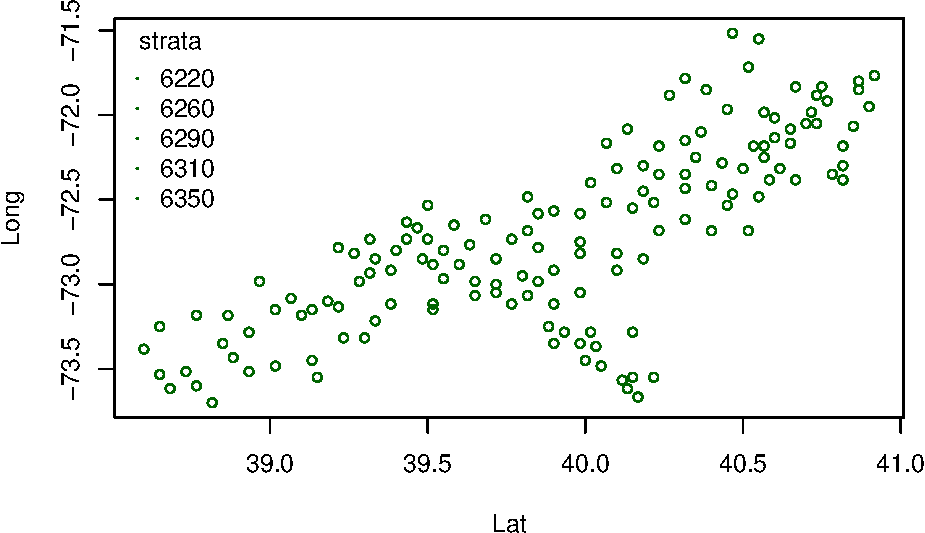
\includegraphics{homework2_files/figure-latex/ex6_basic-1.pdf}

\begin{Shaded}
\begin{Highlighting}[]
\KeywordTok{plot}\NormalTok{(coords, }\DataTypeTok{pch=}\DecValTok{1}\NormalTok{, }\DataTypeTok{cex=}\KeywordTok{sqrt}\NormalTok{(lgcatch)}\OperatorTok{/}\DecValTok{2}\NormalTok{, }\DataTypeTok{col=}\StringTok{"darkgreen"}\NormalTok{, }\DataTypeTok{xlab=}\StringTok{"Lat"}\NormalTok{, }\DataTypeTok{ylab=}\StringTok{"Long"}\NormalTok{)}
\NormalTok{leg.vals <-}\StringTok{ }\KeywordTok{round}\NormalTok{(}\KeywordTok{quantile}\NormalTok{(lgcatch),}\DecValTok{0}\NormalTok{)}
\KeywordTok{legend}\NormalTok{(}\StringTok{"topleft"}\NormalTok{, }\DataTypeTok{pch=}\DecValTok{1}\NormalTok{, }\DataTypeTok{legend=}\NormalTok{leg.vals, }\DataTypeTok{col=}\StringTok{"darkgreen"}\NormalTok{,}
       \DataTypeTok{pt.cex=}\KeywordTok{sqrt}\NormalTok{(leg.vals)}\OperatorTok{/}\DecValTok{1000}\NormalTok{, }\DataTypeTok{bty=}\StringTok{"n"}\NormalTok{, }\DataTypeTok{title=}\StringTok{"lgcatch"}\NormalTok{)}
\end{Highlighting}
\end{Shaded}

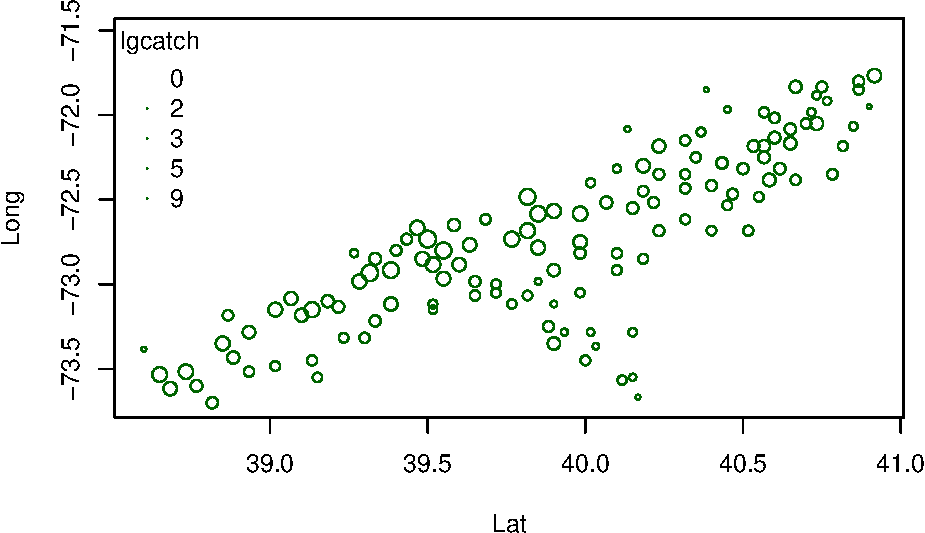
\includegraphics{homework2_files/figure-latex/ex6_basic-2.pdf}

\paragraph{Create a color palette for subsequent
plots.}\label{create-a-color-palette-for-subsequent-plots.}

\begin{Shaded}
\begin{Highlighting}[]
\NormalTok{col.br <-}\StringTok{ }\KeywordTok{colorRampPalette}\NormalTok{(}\KeywordTok{c}\NormalTok{(}\StringTok{"blue"}\NormalTok{, }\StringTok{"cyan"}\NormalTok{, }\StringTok{"yellow"}\NormalTok{, }\StringTok{"red"}\NormalTok{))}
\NormalTok{col.pal <-}\StringTok{ }\KeywordTok{col.br}\NormalTok{(}\DecValTok{5}\NormalTok{)}

\NormalTok{fixed <-}\StringTok{ }\KeywordTok{classIntervals}\NormalTok{(strata, }\DataTypeTok{n =} \DecValTok{4}\NormalTok{, }\DataTypeTok{style =} \StringTok{"fixed"}\NormalTok{, }
                        \DataTypeTok{fixedBreaks =} \KeywordTok{c}\NormalTok{(}\DecValTok{0}\NormalTok{,}\DecValTok{6260}\NormalTok{, }\DecValTok{62290}\NormalTok{, }\DecValTok{6310}\NormalTok{, }\KeywordTok{max}\NormalTok{(strata) }\OperatorTok{+}\StringTok{ }\DecValTok{1}\NormalTok{))}
\NormalTok{fixed.col <-}\StringTok{ }\KeywordTok{findColours}\NormalTok{(fixed, col.pal)}
\KeywordTok{plot}\NormalTok{(coords, }\DataTypeTok{col =}\NormalTok{ fixed.col, }\DataTypeTok{pch =} \DecValTok{19}\NormalTok{, }\DataTypeTok{cex =} \FloatTok{0.5}\NormalTok{, }
     \DataTypeTok{main =} \StringTok{"strata classes"}\NormalTok{, }\DataTypeTok{xlab =} \StringTok{"Lat"}\NormalTok{, }\DataTypeTok{ylab =} \StringTok{"Long"}\NormalTok{)}
\KeywordTok{legend}\NormalTok{(}\StringTok{"topleft"}\NormalTok{, }\DataTypeTok{fill =} \KeywordTok{attr}\NormalTok{(fixed.col, }\StringTok{"palette"}\NormalTok{),}
       \DataTypeTok{legend =} \KeywordTok{c}\NormalTok{(}\StringTok{"strata1"}\NormalTok{, }\StringTok{"strata2"}\NormalTok{, }\StringTok{"strata3"}\NormalTok{, }\StringTok{"strata4"}\NormalTok{), }
       \DataTypeTok{bty =} \StringTok{"n"}\NormalTok{)}
\end{Highlighting}
\end{Shaded}

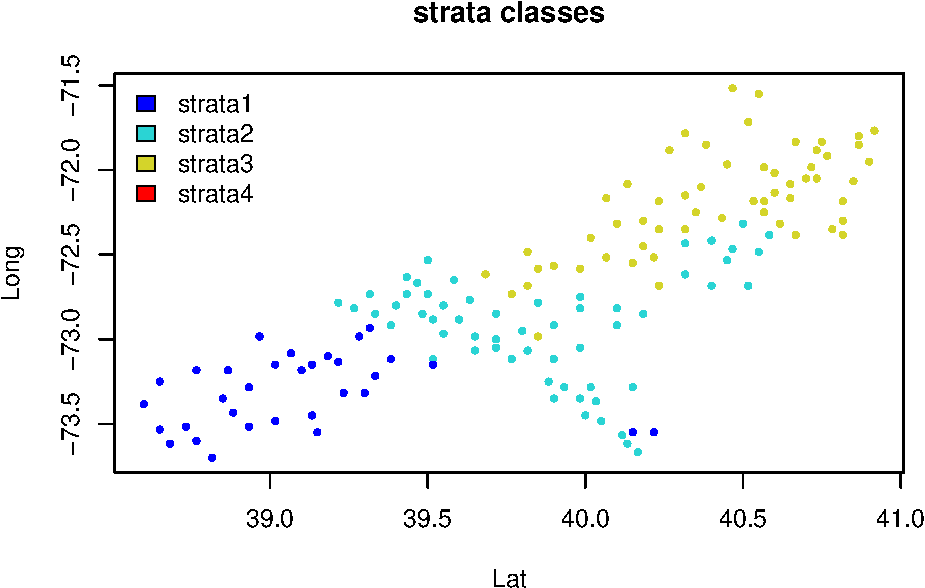
\includegraphics{homework2_files/figure-latex/ex6_color-1.pdf}

\paragraph{Surface}\label{surface}

\begin{Shaded}
\begin{Highlighting}[]
\NormalTok{## MBA and fields libraries for creating surface interpolation plots}
\NormalTok{x.res <-}\StringTok{ }\DecValTok{148}
\NormalTok{y.res <-}\StringTok{ }\DecValTok{148}
\NormalTok{surf <-}\StringTok{ }\KeywordTok{mba.surf}\NormalTok{(}\KeywordTok{cbind}\NormalTok{(coords, strata), }
                 \DataTypeTok{no.X =}\NormalTok{ x.res, }\DataTypeTok{no.Y =}\NormalTok{ y.res, }
                 \DataTypeTok{h =} \DecValTok{5}\NormalTok{, }\DataTypeTok{m =} \DecValTok{2}\NormalTok{, }\DataTypeTok{extend =} \OtherTok{FALSE}\NormalTok{)}\OperatorTok{$}\NormalTok{xyz.est}
\KeywordTok{image.plot}\NormalTok{(surf, }\DataTypeTok{xaxs =} \StringTok{"r"}\NormalTok{, }
           \DataTypeTok{yaxs =} \StringTok{"r"}\NormalTok{, }\DataTypeTok{xlab =} \StringTok{"lat"}\NormalTok{, }
           \DataTypeTok{ylab =} \StringTok{"long"}\NormalTok{, }\DataTypeTok{col =} \KeywordTok{col.br}\NormalTok{(}\DecValTok{25}\NormalTok{))}
\KeywordTok{contour}\NormalTok{(surf, }\DataTypeTok{add=}\NormalTok{T) }
\end{Highlighting}
\end{Shaded}

\includegraphics{homework2_files/figure-latex/Surface-1.pdf}

\paragraph{3D Plot}\label{d-plot}

\begin{Shaded}
\begin{Highlighting}[]
\KeywordTok{library}\NormalTok{(rgl)}
\NormalTok{col <-}\StringTok{ }\KeywordTok{rbind}\NormalTok{(}\DecValTok{0}\NormalTok{, }\KeywordTok{cbind}\NormalTok{(}\KeywordTok{matrix}\NormalTok{(}\KeywordTok{drape.color}\NormalTok{(surf[[}\DecValTok{3}\NormalTok{]],}
                                         \DataTypeTok{col =} \KeywordTok{col.br}\NormalTok{(}\DecValTok{25}\NormalTok{)), x.res }\OperatorTok{-}\StringTok{ }\DecValTok{1}\NormalTok{, y.res}\OperatorTok{-}\DecValTok{1}\NormalTok{), }\DecValTok{0}\NormalTok{))}
\KeywordTok{surface3d}\NormalTok{(surf[[}\DecValTok{1}\NormalTok{]], surf[[}\DecValTok{2}\NormalTok{]], surf[[}\DecValTok{3}\NormalTok{]], }\DataTypeTok{col =} \KeywordTok{abs}\NormalTok{(col))}
\KeywordTok{axes3d}\NormalTok{()}

\KeywordTok{title3d}\NormalTok{(}\DataTypeTok{main =} \StringTok{"strata"}\NormalTok{, }\DataTypeTok{xlab =} \StringTok{"Lat"}\NormalTok{, }\DataTypeTok{ylab =} \StringTok{"Long"}\NormalTok{, }\DataTypeTok{zlab =} \StringTok{"Strata"}\NormalTok{)}
\KeywordTok{drape.plot}\NormalTok{(surf[[}\DecValTok{1}\NormalTok{]], surf[[}\DecValTok{2}\NormalTok{]], surf[[}\DecValTok{3}\NormalTok{]],}
           \DataTypeTok{col =} \KeywordTok{col.br}\NormalTok{(}\DecValTok{150}\NormalTok{), }\DataTypeTok{theta =} \DecValTok{225}\NormalTok{, }\DataTypeTok{phi =} \DecValTok{50}\NormalTok{,}
           \DataTypeTok{border =} \OtherTok{FALSE}\NormalTok{, }\DataTypeTok{add.legend =} \OtherTok{FALSE}\NormalTok{,}
           \DataTypeTok{xlab =} \StringTok{"Lat"}\NormalTok{, }\DataTypeTok{ylab =} \StringTok{"Long"}\NormalTok{, }\DataTypeTok{zlab =} \StringTok{"Strata"}\NormalTok{)}
\KeywordTok{image.plot}\NormalTok{(}\DataTypeTok{zlim =} \KeywordTok{range}\NormalTok{(surf[[}\DecValTok{3}\NormalTok{]], }\DataTypeTok{na.rm =} \OtherTok{TRUE}\NormalTok{),}
           \DataTypeTok{legend.only =} \OtherTok{TRUE}\NormalTok{, }\DataTypeTok{horizontal =} \OtherTok{FALSE}\NormalTok{)}
\end{Highlighting}
\end{Shaded}

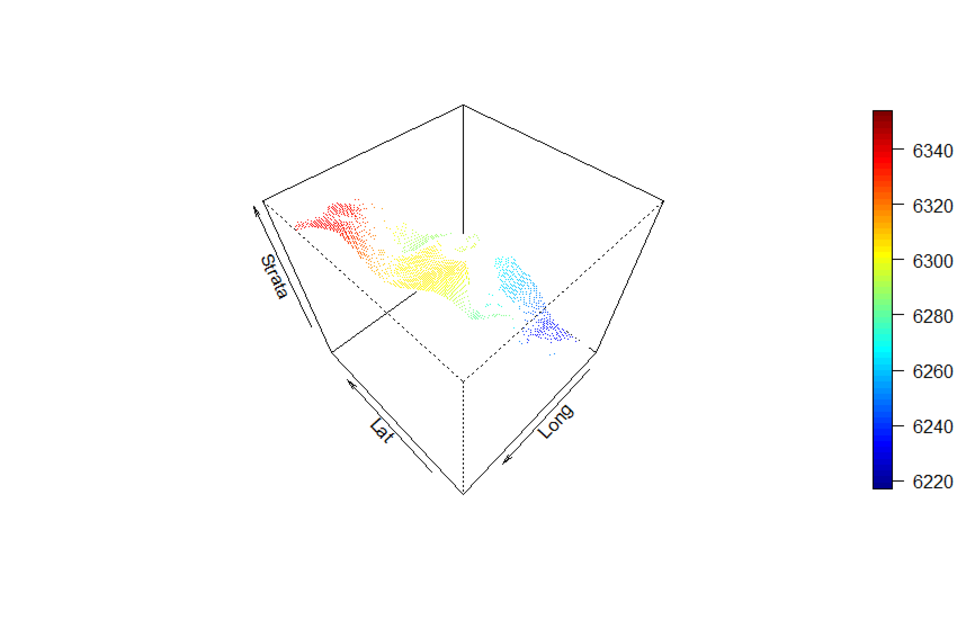
\includegraphics{homework2_files/figure-latex/ex6_3dd-1.pdf}

\subsubsection{(a)}\label{a}

\begin{Shaded}
\begin{Highlighting}[]
\CommentTok{#*********R CODE START************}
\KeywordTok{summary}\NormalTok{(myscallops)}
\end{Highlighting}
\end{Shaded}

\begin{verbatim}
##      strata         sample           lat             long       
##  Min.   :6220   Min.   :  1.0   Min.   :38.60   Min.   :-73.70  
##  1st Qu.:6260   1st Qu.:106.8   1st Qu.:39.46   1st Qu.:-73.14  
##  Median :6290   Median :147.0   Median :39.98   Median :-72.74  
##  Mean   :6288   Mean   :131.8   Mean   :39.91   Mean   :-72.72  
##  3rd Qu.:6310   3rd Qu.:185.2   3rd Qu.:40.41   3rd Qu.:-72.31  
##  Max.   :6350   Max.   :224.0   Max.   :40.92   Max.   :-71.52  
##      tcatch           prerec           recruits          lgcatch     
##  Min.   :   0.0   Min.   :   0.00   Min.   :   0.00   Min.   :0.000  
##  1st Qu.:   8.0   1st Qu.:   1.00   1st Qu.:   5.00   1st Qu.:2.197  
##  Median :  30.0   Median :   8.00   Median :  21.50   Median :3.434  
##  Mean   : 274.6   Mean   : 156.55   Mean   : 118.06   Mean   :3.483  
##  3rd Qu.: 115.2   3rd Qu.:  48.25   3rd Qu.:  73.75   3rd Qu.:4.756  
##  Max.   :7084.0   Max.   :4487.00   Max.   :2597.00   Max.   :8.866
\end{verbatim}

\subsubsection{(b)}\label{b}

\begin{Shaded}
\begin{Highlighting}[]
\CommentTok{#*********R CODE START************}


\NormalTok{max.dist <-}\StringTok{ }\FloatTok{0.25} \OperatorTok{*}\StringTok{ }\KeywordTok{max}\NormalTok{(}\KeywordTok{iDist}\NormalTok{(coords))}
\NormalTok{bins <-}\StringTok{ }\DecValTok{50}
\NormalTok{vario.strata <-}\StringTok{ }\KeywordTok{variog}\NormalTok{(}\DataTypeTok{coords =}\NormalTok{ coords,}
                       \DataTypeTok{data =}\NormalTok{ myscallops}\OperatorTok{$}\NormalTok{strata,}
                       \DataTypeTok{uvec =}\NormalTok{ (}\KeywordTok{seq}\NormalTok{(}\DecValTok{0}\NormalTok{, max.dist, }\DataTypeTok{length =}\NormalTok{ bins)))}
\end{Highlighting}
\end{Shaded}

\begin{verbatim}
## variog: computing omnidirectional variogram
\end{verbatim}

\begin{Shaded}
\begin{Highlighting}[]
\KeywordTok{plot}\NormalTok{(vario.strata,}\DataTypeTok{type=}\StringTok{"o"}\NormalTok{)}
\end{Highlighting}
\end{Shaded}

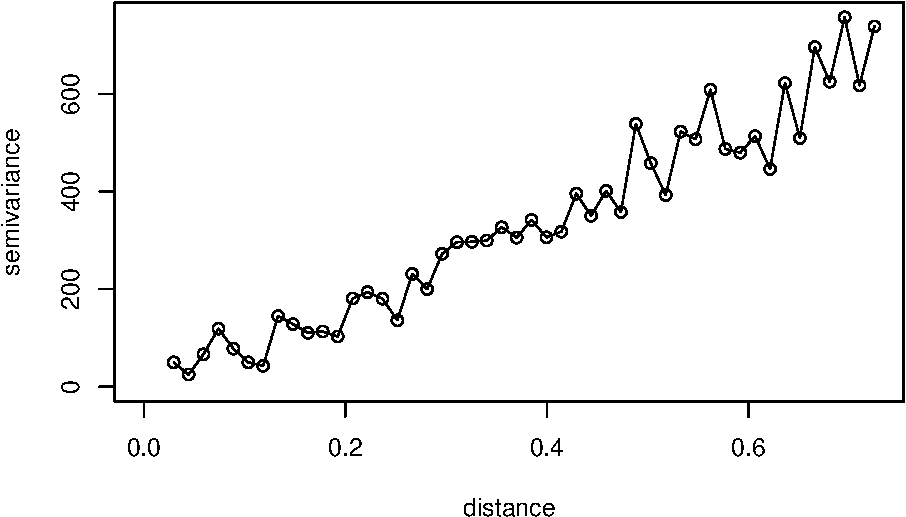
\includegraphics{homework2_files/figure-latex/ex_b-1.pdf}

\subsubsection{(c)}\label{c}

\begin{Shaded}
\begin{Highlighting}[]
\CommentTok{#*********R CODE START************}
\NormalTok{fit.strata<-}\StringTok{ }\KeywordTok{variofit}\NormalTok{(vario.strata,}\DataTypeTok{cov.model=}\StringTok{"exponential"}\NormalTok{,}\DataTypeTok{fix.nugget=}\OtherTok{FALSE}\NormalTok{, }\DataTypeTok{nugget=}\DecValTok{18}\NormalTok{)}
\end{Highlighting}
\end{Shaded}

\begin{verbatim}
## variofit: covariance model used is exponential 
## variofit: weights used: npairs 
## variofit: minimisation function used: optim
\end{verbatim}

\begin{verbatim}
## Warning in variofit(vario.strata, cov.model = "exponential", fix.nugget =
## FALSE, : initial values not provided - running the default search
\end{verbatim}

\begin{verbatim}
## variofit: searching for best initial value ... selected values:
##               sigmasq  phi    tausq kappa
## initial.value "757.26" "0.58" "18"  "0.5"
## status        "est"    "est"  "est" "fix"
## loss value: 30162508.5201582
\end{verbatim}

\begin{Shaded}
\begin{Highlighting}[]
\NormalTok{fit.strata}
\end{Highlighting}
\end{Shaded}

\begin{verbatim}
## variofit: model parameters estimated by WLS (weighted least squares):
## covariance model is: exponential
## parameter estimates:
##      tausq    sigmasq        phi 
##       0.00 1520154.43    1685.73 
## Practical Range with cor=0.05 for asymptotic range: 5049.997
## 
## variofit: minimised weighted sum of squares = 12635537
\end{verbatim}

As we can see above\$nugget=tausq=0\$\\
\(sill=tausq+sigmasq=3439272.97\)\\
\(range=3813.02\)

\subsection{Excerse 7}\label{excerse-7}

\begin{Shaded}
\begin{Highlighting}[]
\CommentTok{#*********R CODE START************}
\NormalTok{url_coal <-}\StringTok{ "https://www.counterpointstat.com/uploads/1/1/9/3/119383887/coal.ash.txt"}
\NormalTok{coalash <-}\StringTok{ }\KeywordTok{read.table}\NormalTok{(url_coal,}\DataTypeTok{header =}\NormalTok{ T)}
\end{Highlighting}
\end{Shaded}

\subsubsection{(a)}\label{a-1}

\begin{Shaded}
\begin{Highlighting}[]
\CommentTok{#*********R CODE START************}
\NormalTok{coords_coal <-}\StringTok{ }\KeywordTok{as.matrix}\NormalTok{(coalash[,}\KeywordTok{c}\NormalTok{(}\StringTok{"x"}\NormalTok{,}\StringTok{"y"}\NormalTok{)])}
\NormalTok{coal <-}\StringTok{ }\NormalTok{coalash}\OperatorTok{$}\NormalTok{coal}
\NormalTok{x.res <-}\StringTok{ }\DecValTok{208}
\NormalTok{y.res <-}\StringTok{ }\DecValTok{208}
\NormalTok{surf <-}\StringTok{ }\KeywordTok{mba.surf}\NormalTok{(}\KeywordTok{cbind}\NormalTok{(coords_coal, coal),}
                 \DataTypeTok{no.X =}\NormalTok{ x.res, }\DataTypeTok{no.Y =}\NormalTok{ y.res, }
                 \DataTypeTok{h =} \DecValTok{5}\NormalTok{, }\DataTypeTok{m =} \DecValTok{2}\NormalTok{, }\DataTypeTok{extend =} \OtherTok{FALSE}\NormalTok{)}\OperatorTok{$}\NormalTok{xyz.est}
\KeywordTok{image.plot}\NormalTok{(surf, }\DataTypeTok{xaxs =} \StringTok{"r"}\NormalTok{, }\DataTypeTok{yaxs =} \StringTok{"r"}\NormalTok{, }\DataTypeTok{xlab =} \StringTok{"x"}\NormalTok{, }\DataTypeTok{ylab =} \StringTok{"y"}\NormalTok{)}
\KeywordTok{contour}\NormalTok{(surf, }\DataTypeTok{add=}\NormalTok{T) }
\end{Highlighting}
\end{Shaded}

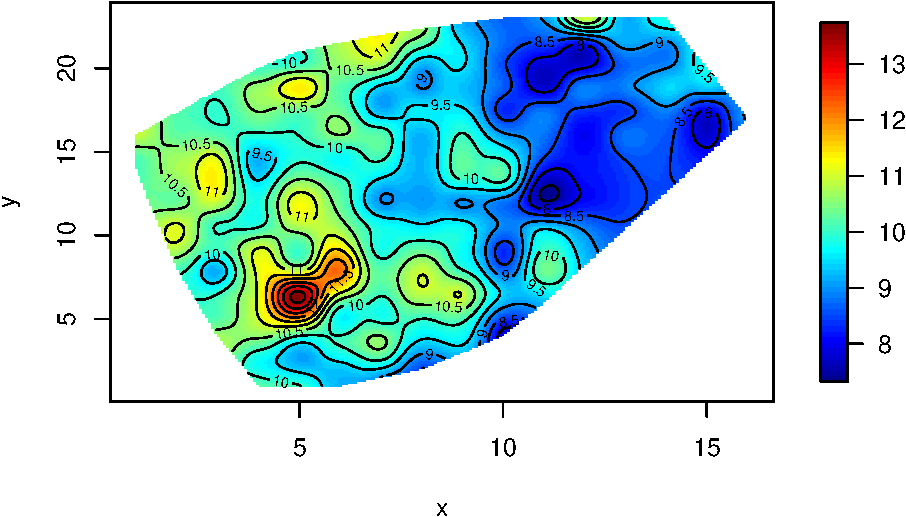
\includegraphics{homework2_files/figure-latex/ex7_a-1.pdf}

\subsubsection{(b)}\label{b-1}

\begin{Shaded}
\begin{Highlighting}[]
\CommentTok{#*********R CODE START************}
\KeywordTok{library}\NormalTok{(ggplot2)}
\NormalTok{coal <-}\StringTok{ }\NormalTok{coalash}\OperatorTok{$}\NormalTok{coal}
\KeywordTok{qplot}\NormalTok{(coal, }\DataTypeTok{geom=}\StringTok{"histogram"}\NormalTok{) }
\end{Highlighting}
\end{Shaded}

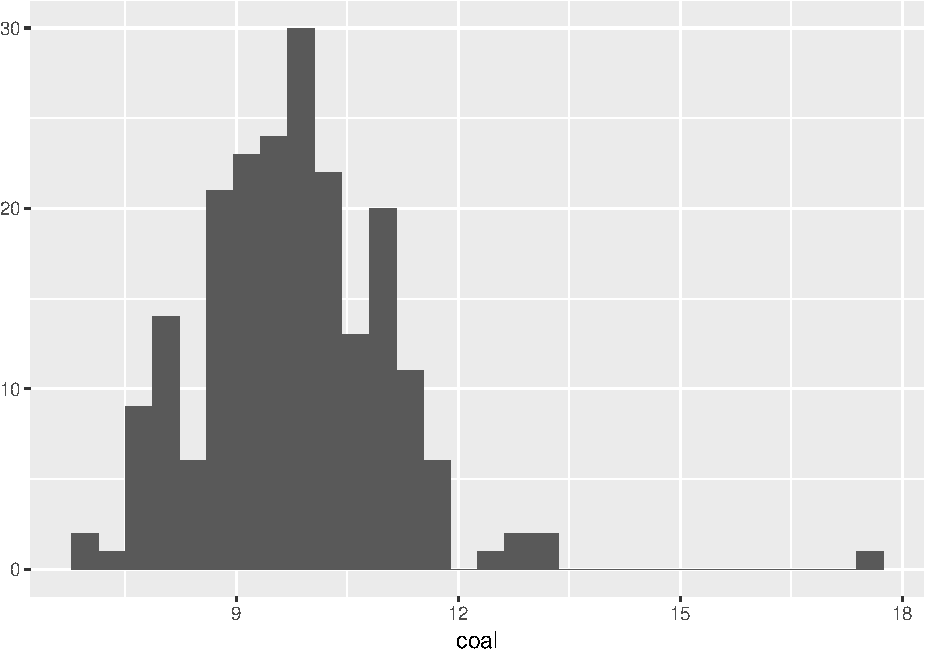
\includegraphics{homework2_files/figure-latex/ex7_b-1.pdf}

\begin{Shaded}
\begin{Highlighting}[]
\KeywordTok{stem}\NormalTok{(coal)}
\end{Highlighting}
\end{Shaded}

\begin{verbatim}
## 
##   The decimal point is at the |
## 
##    7 | 00366678888999
##    8 | 0011122222223556666666788888899999999
##    9 | 00000000111112222223333333344444455555566666666777888888888899999999
##   10 | 00000000111111122222233333444444456666677777788888899999
##   11 | 00001111222222233445666789
##   12 | 578
##   13 | 11
##   14 | 
##   15 | 
##   16 | 
##   17 | 6
\end{verbatim}

\begin{Shaded}
\begin{Highlighting}[]
\KeywordTok{summary}\NormalTok{(coalash)}
\end{Highlighting}
\end{Shaded}

\begin{verbatim}
##        x                y              coal       
##  Min.   : 1.000   Min.   : 1.00   Min.   : 7.000  
##  1st Qu.: 5.000   1st Qu.: 8.00   1st Qu.: 8.960  
##  Median : 7.000   Median :13.00   Median : 9.785  
##  Mean   : 7.534   Mean   :12.91   Mean   : 9.779  
##  3rd Qu.:10.000   3rd Qu.:18.00   3rd Qu.:10.568  
##  Max.   :16.000   Max.   :23.00   Max.   :17.610
\end{verbatim}

\subsubsection{(c)}\label{c-1}

\begin{Shaded}
\begin{Highlighting}[]
\CommentTok{#*********R CODE START************}
\NormalTok{vario.coal <-}\StringTok{ }\KeywordTok{variog}\NormalTok{(}\DataTypeTok{coords =}\NormalTok{ coords_coal,}
                     \DataTypeTok{data =}\NormalTok{ coal, }\DataTypeTok{uvec =}\NormalTok{ (}\KeywordTok{seq}\NormalTok{(}\DecValTok{0}\NormalTok{, }\DataTypeTok{length =}\NormalTok{ bins)))}
\end{Highlighting}
\end{Shaded}

\begin{verbatim}
## variog: computing omnidirectional variogram
\end{verbatim}

\begin{Shaded}
\begin{Highlighting}[]
\KeywordTok{plot}\NormalTok{(vario.coal,}\DataTypeTok{type=}\StringTok{"o"}\NormalTok{)}
\end{Highlighting}
\end{Shaded}

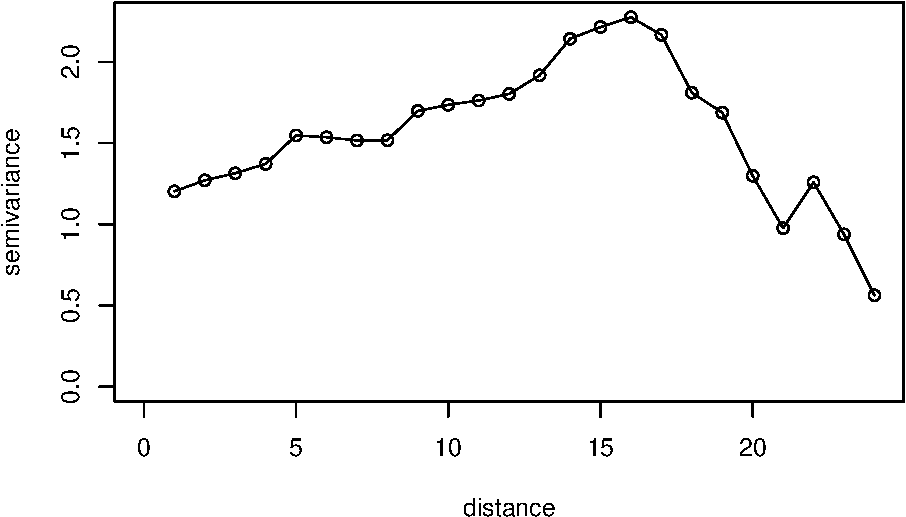
\includegraphics{homework2_files/figure-latex/ex7_c-1.pdf}

\subsubsection{(d)}\label{d}

\begin{Shaded}
\begin{Highlighting}[]
\CommentTok{#*********R CODE START************}
\NormalTok{fit.coal<-}\StringTok{ }\KeywordTok{variofit}\NormalTok{(vario.coal,}
                    \DataTypeTok{cov.model=}\StringTok{"exponential"}\NormalTok{,}
                    \DataTypeTok{fix.nugget=}\OtherTok{FALSE}\NormalTok{,}
                    \DataTypeTok{max.dist =} \DecValTok{1}\OperatorTok{/}\DecValTok{17}\NormalTok{, }\DataTypeTok{nugget=}\FloatTok{1.2}\NormalTok{)}
\end{Highlighting}
\end{Shaded}

\begin{verbatim}
## variofit: covariance model used is exponential 
## variofit: weights used: npairs 
## variofit: minimisation function used: optim
\end{verbatim}

\begin{verbatim}
## Warning in variofit(vario.coal, cov.model = "exponential", fix.nugget =
## FALSE, : initial values not provided - running the default search
\end{verbatim}

\begin{verbatim}
## variofit: searching for best initial value ... selected values:
##               sigmasq phi   tausq kappa
## initial.value "1.14"  "0"   "1.2" "0.5"
## status        "est"   "est" "est" "fix"
## loss value: 0
\end{verbatim}

\begin{Shaded}
\begin{Highlighting}[]
\NormalTok{fit.coal}
\end{Highlighting}
\end{Shaded}

\begin{verbatim}
## variofit: model parameters estimated by WLS (weighted least squares):
## covariance model is: exponential
## parameter estimates:
##   tausq sigmasq     phi 
##  1.2000  1.1375  0.0000 
## Practical Range with cor=0.05 for asymptotic range: 0.0001159668
## 
## variofit: minimised weighted sum of squares = 0
\end{verbatim}

As we can see above, the sill corresponded to round 17 is around 2.24,
which is match to the plot in (b).


\end{document}
